\chapter{基本概念}\label{c1}
\section{复射影平面\texorpdfstring{$P^2\C$}{P2C}上的代数曲线}\label{s1-1}
设$f(x,y)$是实系数多项式, $\R^2$上由
\begin{equation}\label{e1-1-1}
    f(x,y)=0
\end{equation}
给出的图形称为\textit{实代数曲线}, $f(x,y)$的次数称为这代数曲线的\textit{次数}. 读者已经熟悉了一次和二次的实代数曲线, 但是在实数范围内讨论更一般的代数曲线会有若干不方便之处, 这主要是因为实数域不是代数闭域. 例如, 我们欲讨论这样的问题: 一条直线与代数曲线有多少交点. 不妨设直线过原点, 它的参数方程可以写成\begin{equation}\label{e1-1-2}
    \begin{cases}
        x=\alpha t, \\
        y=\beta t. 
    \end{cases}
\end{equation}
设
\[f(x,y)=f_n(x,y)+f_{n-1}(x,y)+\cdots+f_0, \]
其中$f_k(x,y)$ 是$k$次齐次多项式. 把\eqref{e1-1-2}代入\eqref{e1-1-1}得
\begin{equation}\label{e1-1-3}
    f_n(\alpha,\beta)t^n+f_{n-1}(\alpha,\beta)t^{n-1}+\cdots+f_0=0. 
\end{equation}
在实数范围内要判断这样的方程有多少根不是一件容易的事, 但是如果考虑复系数的$f(x,y)$并把\eqref{e1-1-1}看成$\C^2$上的代数曲线, 再来讨论复直线与复代数曲线的交点, 也得到\eqref{e1-1-3}. 由熟知的代数基本定理, 只要$f_n(\alpha,\beta)\neq0$, \eqref{e1-1-3}恰有$n$个根(记重数). In other words, the complex algebraic curve $C$ of degree $n$ and the complex line $L$ intersect at $n$ points (the intersection points corresponding to multiple roots are thought of as multiple points of intersection). There is one exception to the preceding discussion: if 
\begin{gather*}
    f_n(\alpha,\beta)=f_{n-1}(\alpha,\beta)=\cdots=f_{m+1}(\alpha,\beta)=0, \\
    f_m(\alpha,\beta)\neq0, 
\end{gather*}
then $L$ and $C$ intersect in only $m$ points in $\C^2$. In this case we may regard the remaining $n-m$ points of intersection as being at infinity. This viewpoint can be explained in more detail as follows: substituting $1/s$ for $t$ in \eqref{e1-1-3} and multiplicity both sides of the equation by $s^n$, we have 
\begin{equation}\label{e1-1-3-2}\tag{\ref*{e1-1-3}$'$}
    f_n(\alpha,\beta)+f_{n-1}(\alpha,\beta)s+\cdots+f_0(\alpha,\beta)s^n=0. 
\end{equation}
If $f_n(\alpha,\beta)\neq0$, then $s=0$ (which corresponding to $t=\infty$) is not a root of \eqref{e1-1-3-2}; if 
\begin{gather*}
    f_n(\alpha,\beta)=f_{n-1}(\alpha,\beta)=\cdots=f_{m+1}(\alpha,\beta)=0, \\
    f_m(\alpha,\beta)\neq0, 
\end{gather*}
then $s=0$ (corresponding to $t=\infty$) is a root of \eqref{e1-1-3-2} of multiplicity $n-m$. We then say that $L$ and $C$ have a point of intersection of multiplicity $n-m$ at infinity. Hence, for the convenience of our discussion, we must add ``a line at infinity'' to $\C^2$, thereby arriving at the complex projective plane $P^2\C$. 

The most convenient way of adding a line at infinity to $\C^2$ is through the use of homogeneous coordinates. For a point $(x,y)\in\C^2$, its \textit{homogeneous coordinates} are any set of complex numbers $(\zeta,\xi,\eta)$ satisfying 
\begin{equation}\label{e1-1-4}
    x=\xi/\zeta, \quad y=\eta/\zeta. 
\end{equation}
If $(\zeta,\xi,\eta)$ are homogeneous coordinates for $(x,y)$, then clearly so are $(\lambda\zeta,\lambda\xi,\lambda\eta)$ $(\lambda\in\C,\lambda\neq0)$. In order for \eqref{e1-1-4} to be well defined, it is necessary that $\zeta\neq0$. However, if $\xi$ and $\eta$ are not both $0$, then as $\zeta\to0$ the points $x=\xi/\zeta$, $y=\eta/\zeta$ approach infinity in the direction $\xi:\eta$. Therefore we can let $(0,\xi,\eta)$ denote the point at infinity along the direction $\xi:\eta$. In this way, through homogeneous coordinates we can add a point at infinity to each direction in $\C^2$, and the set of all such points at infinity is called the \textit{line at infinity}, $L_\infty$. $\C^2$ together with $L_\infty$ is called the complex projective plane $P^2\C$. We now describe this process more rigorously in the following. 

In the set $\C^3\backslash\{(0,0,0)\}$ we introduce a relation $\sim$ as follows: 
\begin{equation}\label{e1-1-5}
    \begin{gathered}
        (\zeta,\xi,\eta)\sim(\zeta',\xi',\eta')\\
        \text{if and only if such that $\exists\lambda\in\C$, $\lambda\neq0$ such that}\\
        \zeta'=\lambda\zeta, \ \xi'=\lambda\xi, \ \eta'=\lambda\eta. 
    \end{gathered}
\end{equation}
This is obviously an equivalence relation. Accordingly, we divide $\C^3\backslash\{(0,0,0)\}$ into equivalence classes, and the equivalence class containing $(\zeta,\xi,\eta)$ is denoted by $[\zeta,\xi,\eta]$. clearly
\[[\zeta,\xi,\eta]=[\lambda\zeta,\lambda\xi,\lambda\eta]\quad\forall\lambda\in\C\backslash\{0\}. \]
The quotient space induced by this equivalence relation (the space of equivalence classes), 
\[(\C^3\backslash\{(0,0,0)\})/\sim\]
is called the \textit{complex projective plane} and is denoted by $P^2\C$ (or simply $\P^2$ when there is no danger of confusion). As a quotient space, $P^2\C$ possesses a quotient topology. We shall arrive at a better understanding of $P^2\C$ when we discuss its complex manifold structure in \autoref{s1-7}. 

Let us now examine the representation in homogeneous coordinates of the curve $C$ given by \eqref{e1-1-1}. Substituting 
\[x=\xi/\zeta, \quad y=\eta/\zeta\]
into \eqref{e1-1-1} and multiplying both sides of the resulting expression by $\zeta^n$, we obtain 
\[F(\zeta,\xi,\eta)=f_n(\xi,\eta)+f_{n-1}(\xi,\eta)\zeta+\cdots+f_0\zeta^n=0. \]
The left side of this equation is a homogeneous polynomial in $\zeta,\xi,\eta$. In general, if $F(\zeta,\xi,\eta)$ is a homogeneous polynomial in $\zeta,\xi,\eta$, then 
\begin{equation}\label{e1-1-6}
    F(\zeta,\xi,\eta)=0
\end{equation}
represents an \textit{algebraic curve} in $P^2\C$, and the degree of $F$ is called the \textit{degree} of this curve. Equation \eqref{e1-1-6} is called the \textit{homogeneous equation} of this curve. If we restrict ourselves to $\C^2$, then this curve satisfies the \textit{affine equation} 
\begin{equation}\label{e1-1-7}
    f(x,y)=0, 
\end{equation}
where 
\[f(x,y)=F(1,x,y). \]

In this way, the homogeneous equation of a curve determine the affine equation of this curve. On the other hand, the degree of the curve and its affine equation uniquely determine its homogeneous equation 
\[F(\zeta,\xi,\eta)=0\]
where 
\[F(\zeta,\xi,\eta)=\zeta^n f(\xi/\zeta,\eta/\zeta). \]

If an algebraic curve $C$ is given by 
\[F(\zeta,\xi,\eta)=0, \]
and $F$ decomposes into the product of irreducible homogeneous polynomials 
\[F=F_1^{m_1}F_2^{m_2}\cdots F_l^{m_l}, \]
then we write 
\[C=m_1C_1+m_2C_2+\cdots+m_lC_l\]
where 
\[C_j=\{[\zeta,\xi,\eta]|F_j(\zeta,\xi,\eta)=0\}\ (j=1,2,\cdots,l). \]
Each $C_j$ is called an \textit{irreducible component} of $C$. In the special case when $F$ itself is irreducible, then $C$ is called an \textit{irreducible curve}. 

\section{Riemann面}\label{s1-2}
There exists a close relationship between the study of compect Riemann surfaces and that of algebraic curves: any irreducible plane algebraic curve admits a holomorphic parametric representation and the domain of definition of this representation is a compect Riemann surface. More precisely, we have the following \textit{normalization theorem} (its proof will be given in the next chapter). 
\begin{theorem}
    For any irreducible algebraic curve $C\subset P^2\C$, there exists a compect Riemann surface $\widetilde{C}$ and a holomorphic mapping 
    \[\sigma:\widetilde{C}\to P^2\C\]
    such that $\sigma(\widetilde{C})=C$, and $\sigma$ is injective on the inverse image of the set of smooth points of $C$. 
\end{theorem}

Such a compect Riemann surface $\widetilde{C}$ together with the holomorphic mapping $\sigma$ as above, is called the \textit{normalization} of $C$. Normalization is a powerful tool in the study of algebraic curves. 

On the other hand, any compect Riemann surface can be represented by an algebraic curve. This is another basic fact which we shall be using throughout this book: 
\begin{theorem}
    Any compect Riemann surface $\widetilde{C}$ can be obtained through the normalization of a certain plane algebraic curve $C$ with at most ordinary double points (for the precise definition, see \autoref{s2-1}). That is to say, there exists a holomorphic mapping $\sigma:\widetilde{C}\to P^2\C$, such that $\sigma(\widetilde{C})$ is an algebraic curve possessing at most ordinary double points. \footnote{One proof of this theorem makes use of the theory of sheaf cohomology. The discussion in the appendix of this book outlines the proof; for a complete proof, refer to either \cite[chapter 2]{MR1288523} or \cite[section 5.21]{MR703513}.}
\end{theorem}

From this we see that the study of compect Riemann surfaces and that of plane algebraic curves are in fact the same thing. These two topics form the kernel of this book. In this section, we begin by giving the definition of a Riemann surface and the related basic results on topological classification. 
\begin{definition}
    A \textit{Riemann surface} is a connected Hausdorff topological space $C$ together with an open covering $\{U_\alpha\}$ of $C$ and a family of mappings 
    \[z_\alpha:U_\alpha\to\C\]
    such that
    \begin{enumerate}
        \item each $z_\alpha:U_\alpha\to\C$ is a homeomorphism of $U_\alpha$ onto an open subset of $\C$; 
        \item if $U_\alpha\cap U_\beta\neq\varnothing$, then the function 
        \[z_\beta\circ z_\alpha^{-1}:z_\alpha(U_\alpha\cap U_\beta)\to z_\beta(U_\alpha\cap U_\beta)\]
        is biholomorphic (i.e., the function itself as well as its inverse are both holomorphic). 
        \[\begin{tikzcd}
            &U_\alpha\cap U_\beta\arrow[ld,"z_\alpha"]\arrow[rd,"z_\beta"]&\\
            z_\alpha(U_\alpha\cap U_\beta)\arrow[rr,"z_\beta\circ z_\alpha^{-1}",shift left=.5ex]&&z_\beta(U_\alpha\cap U_\beta\arrow[ll,"z_\alpha\circ z_\beta^{-1}",shift left=.5ex])
        \end{tikzcd}\]
    \end{enumerate}
    We call such a $(U_\alpha,z_\alpha)$ a local holomorphic coordinate, and $\{(U_\alpha,z_\alpha)\}$ a holomorphic coordinate covering. 
\end{definition}

The main topic of this book is the study of compect Riemann surfaces, that is to say, Riemann surfaces which as topological spaces are compect. 
\begin{example}[The set of extended complex numbers $\Sigma=\C\cup\{\infty\}$ (one point compactification of complex numbers)]
    $\Sigma$ is obviously a compect, connected Hausdorff topological space. Now consider the covering $\{U_0,U_1\}$: 
    \[U_0=\Sigma\backslash\{\infty\}=\C, \quad U_1=\Sigma\backslash\{0\}\]
    and the mapping 
    \begin{align*}
        z_0:U_0&\to\C, \\
        z&\mapsto z; \\
        z_1:U_1&\to\C, \\
        z&\mapsto\begin{cases}
            0&z=\infty, \\
            1/z&z\neq\infty. 
        \end{cases}
    \end{align*}
    clearly
    \begin{align*}
        z_1\circ z_0^{-1}:\C\backslash\{0\}&\to\C\backslash\{0\}, \\
        z&\mapsto1/z
    \end{align*}
    is biholomorphic, and likewise $z_0\circ z_1^{-1}$. In this way $\Sigma$ becomes a compact Riemann surface. 

    Since we can identify the unit sphere $S$ with $\Sigma$ through stereographic projection, $S$ therefore also naturally becomes a Riemann surface, called the \textit{Riemann sphere}. The precise coordinate representation is as follows: let $N=(0,0,1)$ denote the north pole and $P=(0,0,-1)$ denote the south pole. Consider the covering $\{U_0,U_1\}$ of $S$ and the mappings $\Phi_0,\Phi_1$: 
    \begin{gather*}
        U_0=S\backslash\{P\}, \quad\Phi_0:U_0\to\C; \\
        U_1=S\backslash\{N\}, \quad\Phi_1:U_1\to\C. 
    \end{gather*}
    Here $\Phi_0$ represents the stereographic projection from the south pole $P$ to $\C$. Taking its conjugate we have 
    \begin{figure}[h]
        \[\includegraphics{figures/1-1}\]
        \caption{球极投影}
    \end{figure}
    \[\Phi_0(X,Y,Z)=\frac{X-iY}{1+Z}; \]
    $\Phi_1$ represents the stereographic projection from the north pole $N$ to $\C$, and 
    \[\Phi_1(X,Y,Z)=\frac{X+iY}{1-Z}. \]
    Here $X,Y,Z$ denote linear coordinates in $\R^3$. We have 
    \begin{align*}
        \Phi_1\circ\Phi_0^{-1}:\C\backslash\{0\}&\to\C\backslash\{0\}, \\
        z&\mapsto1/z, \\
        \Phi_0\circ\Phi_1^{-1}:\C\backslash\{0\}&\to\C\backslash\{0\}, \\
        z&\mapsto1/z. 
    \end{align*}
    It is clear that $\Phi_1\circ\Phi_0^{-1}$ and $\Phi_0\circ\Phi_1^{-1}$ are both biholomorphic. 

    The Riemann sphere is a compect Riemann surface when it has been constructed by either of the two above procedures, viz., either from the extended complex plane or from the unit sphere obtained by stereographic projection. 
\end{example}
\begin{example}[复环面$\C/\Lambda$]
    设复数$w_1,w_2$实线性无关(即不存在实数$\lambda_1,\lambda_2$, $|\lambda_1|+|\lambda_2|\neq0$, 使得$\lambda_1w_1+\lambda_2w_2=0$). 它们在$\C$上定义了一个\textit{格}. 
    \begin{figure}[h]
        \[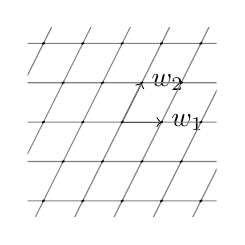
\begin{tikzpicture}[cm={1,0,.5,1,(0,0)}]
            \clip[cm={1,0,-.5,1,(0,0)}](-1.2,-1.2)rectangle(1.2,1.2);
            \draw[->](0,0)--(.5,0)node[right]{$w_1$};
            \draw[->](0,0)--(0,.5)node[right]{$w_2$};
            \draw[thin,gray](-2,-2)grid[step=.5](2,2);
            \foreach\x in{-5,...,5}
            \foreach\y in{-5,...,5}
                \fill(\x*.5,\y*.5)circle[radius=.02];
        \end{tikzpicture}\]
        \caption{格$\Lambda$}
    \end{figure}
    \[\Lambda=\{m_1w_1+m_2w_2|m_1,m_2\in\Z\}. \]
    $\Lambda$ is a discrete subgroup of $\C$ generated by $w_1$ and $w_2$, and is isomorphic to $\Z\oplus\Z$. Now consoder the equivalence relation $\sim$ on $\C$ 
    \[z\sim z'\Leftarrow z-z'\in\Lambda. \]
    The quotient space $C=\C/\Lambda$ of this equivalence relation is called a \textit{complex tours}. It is easily seen that this is a compact, connected Hausdorff topological space. For $\epsilon$ sufficiently small, there exists at most one point of intersection between any disc of radius $\epsilon$ in $\C$ and every equivalence class. 
\end{example}

\section{全纯与半纯函数}\label{s1-3}

\section{全纯与半纯微分}\label{s1-4}

\section{微分形式}\label{s1-5}

\section{Poincar\texorpdfstring{\'e}{e}-Hopf公式}\label{s1-6}

\section{复流形}\label{s1-7}

\section{代数簇}\label{s1-8}

\section{光滑点, 切空间, 隐函数定理}\label{s1-9}

\section{紧Riemann面到复射影空间的全纯映射}\label{s1-10}
